\section{Nyelvek kiválasztása}

\begin{figure}
  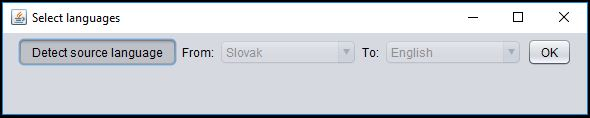
\includegraphics[width=\linewidth]{images/language_selection.jpg}
  \caption{A nyelvválasztó kezelőfelülete}
  \label{fig:language_selection}
\end{figure}

Miután az alkalmazás képes kezelni a fordításokat, a következő lépés a fordítás nyelvének megadása volt. Mivel a szoftver képes nyelvfelismerésre is, ezért a nyelvválasztó funkciót úgy valósítottam meg, hogy a felhasználó képes legyen e funkció be- és kikapcsolására, illetve egyéni nyelvpárok kiválasztására is.  Ez csak azután tehető meg, hogy sikeresen hozzáadunk egy feliratfájlt a lejátszóhoz. Ha ezt megtettük a kezelőfelület elérhető a \textit{Select translator languages} gombra történő kattintással.  Ekkor egy panel nyílik a felhasználó képernyőjére, (\ref{fig:language_selection}) amely egy \textit{JToggleButton}-on kívül kettő \textit{JComboBox}-ot tartalmaz egy \textit{JButton} mellett. Alapesetben a nyelvfelismerés mindig aktív, így a két legördülő listából nem lehet választani. Ez kikapcsolható a \textit{Detect languages} gombra való kattintással. Ekkor elérhetővé válik a két lista is, ahol tetszőlegesen választhatunk a fordító által támogatott nyelvek közül. Választás után az \textit{OK} kattintva az alkalmazás elmenti a kiválasztott elemeket, tehát, ha bezárjuk az ablakot, majd ismét megnyitjuk azt, az eredmény a bezárás előtti állapottal megegyező. Így a megjelenített opciók mindig az aktuális, mentett konfigurációt tükrözik. A fordítás nyelvének megváltoztatása akár filmnézés közben is elvégezhető, nem szükséges hozzá a tartalom újratöltése, azonban minden új feliratfájl lejátszóhoz történő hozzáadása alaphelyzetbe állítja a kiválasztott nyelveket. Az \textit{API} által támogatott nyelvek listája rendkívül széles, a legtöbb ismert nyelvet támogatja.

Mivel az \textit{API} nyelvkódokat használ a nyelvek azonosítására, például \textit{"hu"}, viszont a felhasználó számára megjelenített nyelvek teljes értékű szavak, például \textit{"Hungarian"}, szükség volt ezek összekapcsolására. A nyelv-nyelvkód párokat egy \textit{HashMap}-ben tároljuk kulcs-érték páronként, amelyeket minden egyes nyelvállításkor megvizsgálunk, és  a kulcs alapján az alkalmazás beállítja az annak megfelelő kódot. (\ref{lst:kulcs_ertek}).

\begin{lstlisting}[caption=Aktuális nyelvek beállítása, language=java, label={lst:kulcs_érték}]
while (it.hasNext()) {
    Map.Entry pair = (Map.Entry) it.next();
    if (pair.getKey().equals(fromComboBox.getSelectedItem())) {
        currentFromLanguage = (String) pair.getValue();
    }
    if (pair.getKey().equals(toComboBox.getSelectedItem())) {
        currentToLanguage = (String) pair.getValue();
    }
    it.remove();
}
\end{lstlisting}

Mint említettem, alapesetben a nyelvdetektálás mindig aktív. Ez azt jelenti, hogy a felhasználónak nem kell a nyelvválasztással foglalkoznia, elvégzi ezt helyette az alkalmazás. Emellett ilyen esetben a célnyelv, azaz az a nyelv amire a fordítás történik, mindig a felhasználó számítógépének rendszernyelve, amelyet az alkalmazás a \textit{user.language} változóból olvas ki. Így a a felhasználó számára legkényelmesebben, legkevesebb konfigurációval, mindemellett nagy pontossággal valószínűsíthető, hogy a fordítás mely két nyelv között fog végbemenni, hiszen az \textit{API} nyelvfelismerő funkciója rendkívül megbízható, illetve legtöbbször az operációs rendszer nyelve megegyezik a felszanálója anyanyelvével.
